Let the straight line pass through the point $\vec{A}=\myvec{2 \\-2}$ and makes an angle of 60$^{\circ}$ with x-axis.\\
So slope of the line, $m=\tan 60^{\circ}=\sqrt{3}$ and the direction vector  $\myvec{1 \\m} = \myvec{1 \\\sqrt{3}}$.\\\\
The vector form of the line passing through the point $\vec{A}=\myvec{2 \\-2}$ along the direction vector  $\myvec{1 \\\sqrt{3}}$ is given by:
\begin{align}
\vec{X}=\myvec{2 \\-2}+ \lambda_1\myvec{1 \\\sqrt{3}}
\end{align} 

The normal vector
\begin{align}
\vec{n}=\myvec{0 \quad -1\\1 \quad 0} \myvec{1 \\m} = \myvec{-\sqrt3\\ 1}
\end{align}
The equation of the line in terms of the normal vector is obtained as
\begin{align}
\vec{n^T}\myvec{x-A}  =0\\
\myvec{-\sqrt3\quad 1}x=\myvec{-\sqrt3\quad 1}A\\
\myvec{-\sqrt3\quad 1}x=\myvec{-\sqrt3\quad 1}\myvec{2 \\-2}\\
\myvec{-\sqrt3\quad 1}x=-2\sqrt{3}-2\\
\myvec{\sqrt3/2\quad -1/2}x=\sqrt{3}+1\\
\myvec{ cos 330^{\circ} \quad sin 330^{\circ}}x= 2.732
\end{align}
See Fig.     \ref{eq:solutions/2/2/2/myfig:1}

\begin{figure}[!ht]
 \begin{center}
  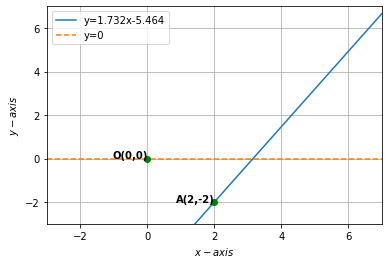
\includegraphics[width=\columnwidth]{solutions/2/2/2/assignment3_fig.png}
    \caption{This is the 2D diagram of the straight line passing through $\myvec{2 \\-2}$ and at an angle of 60$^{\circ}$ with the x axis }
    \label{eq:solutions/2/2/2/myfig:1}
    \end{center}
\end{figure}
